%!TeX root=../pridetop.tex
\chapter[Chapter \thechapter]{}
	
\begin{figure}[t!]
\centering
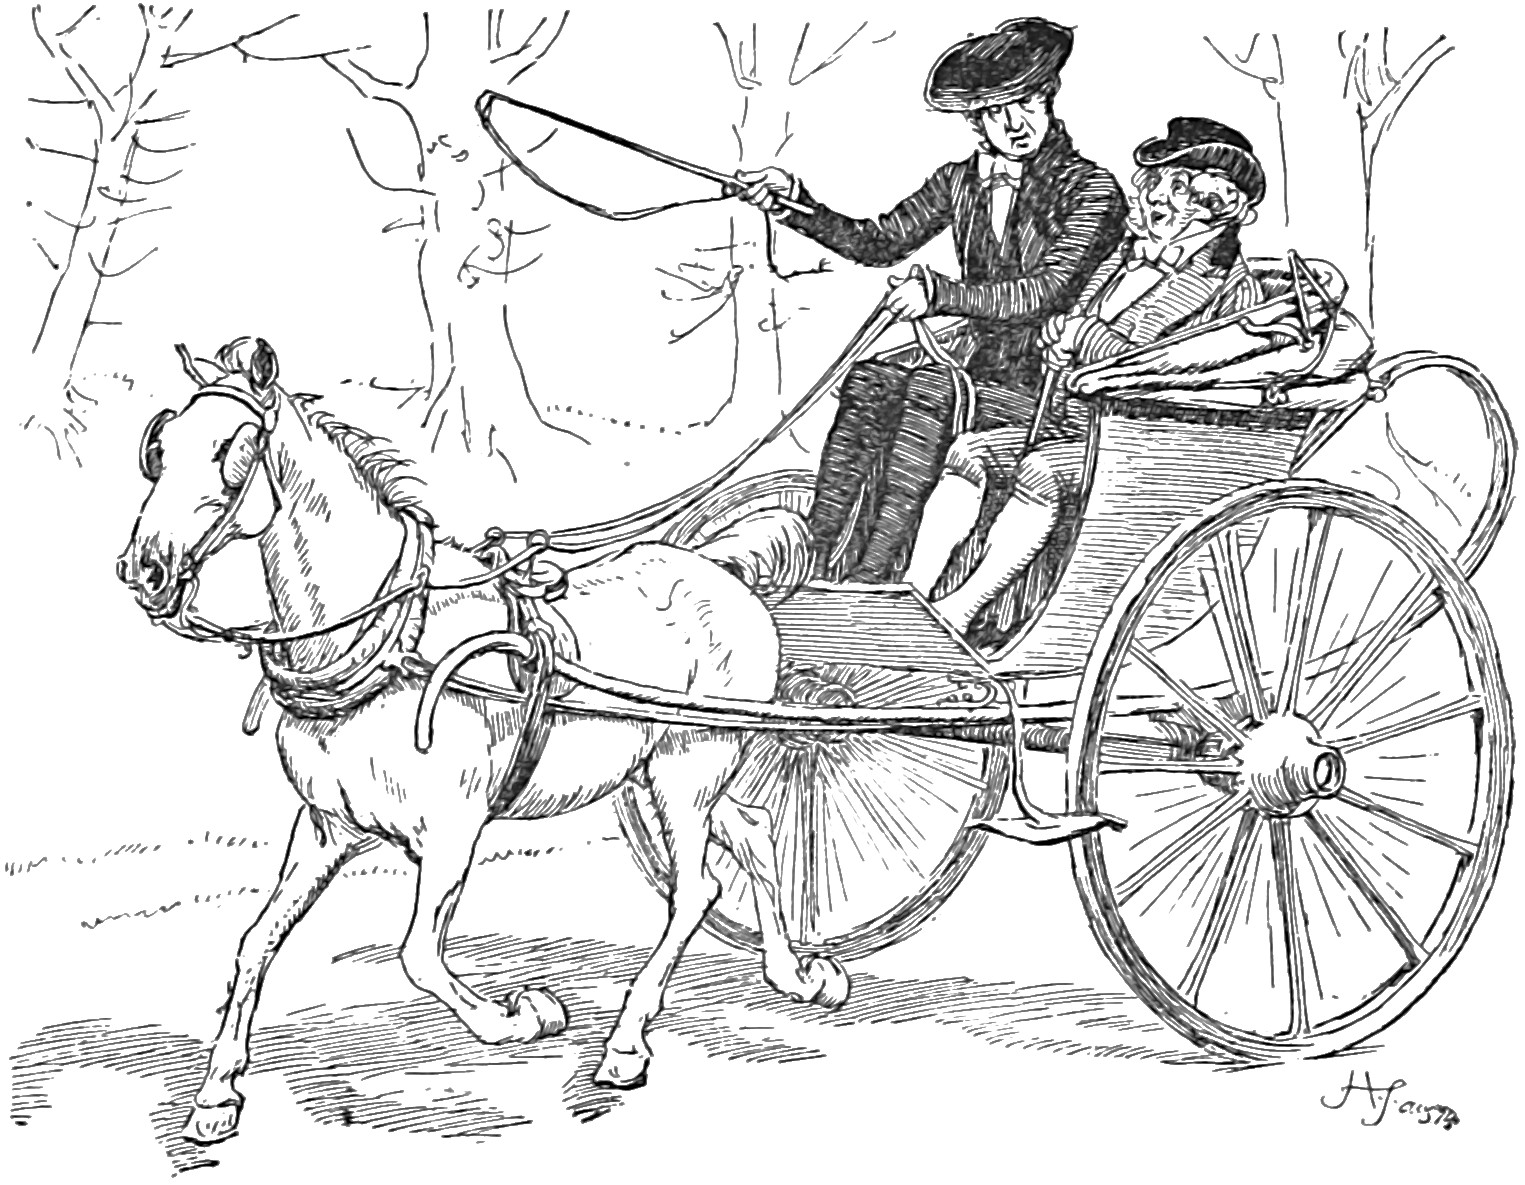
\includegraphics[width=\linewidth]{30top}
\captionlistentry{Headpiece to Chapter \thechapter}
\end{figure}


\lettrine[lines=6,image=true]{initials/chap30s}{ir}  William stayed only a week at Hunsford; but his visit was long enough to convince him of his daughter's being most comfortably settled, and of her possessing such a husband and such a neighbour as were not often met with. While Sir William was with them, Mr Collins devoted his mornings to driving him out in his gig, and showing him the country: but when he went away, the whole family returned to their usual employments, and Elizabeth was thankful to find that they did not see more of her cousin by the alteration; for the chief of the time between breakfast and dinner was now passed by him either at work in the garden, or in reading and writing, and looking out of window in his own book room, which fronted the road. The room in which the ladies sat was backwards. Elizabeth at first had rather wondered that Charlotte should not prefer the dining parlour for common use; it was a better sized room, and had a pleasanter aspect: but she soon saw that her friend had an excellent reason for what she did, for Mr Collins would undoubtedly have been much less in his own apartment had they sat in one equally lively; and she gave Charlotte credit for the arrangement.

From the drawing-room they could distinguish nothing in the lane, and were indebted to Mr Collins for the knowledge of what carriages went along, and how often especially Miss de Bourgh drove by in her phaeton, which he never failed coming to inform them of, though it happened almost every day. She not unfrequently stopped at the Parsonage, and had a few minutes' conversation with Charlotte, but was scarcely ever prevailed on to get out.

\begin{figure}[tbh]
\centering
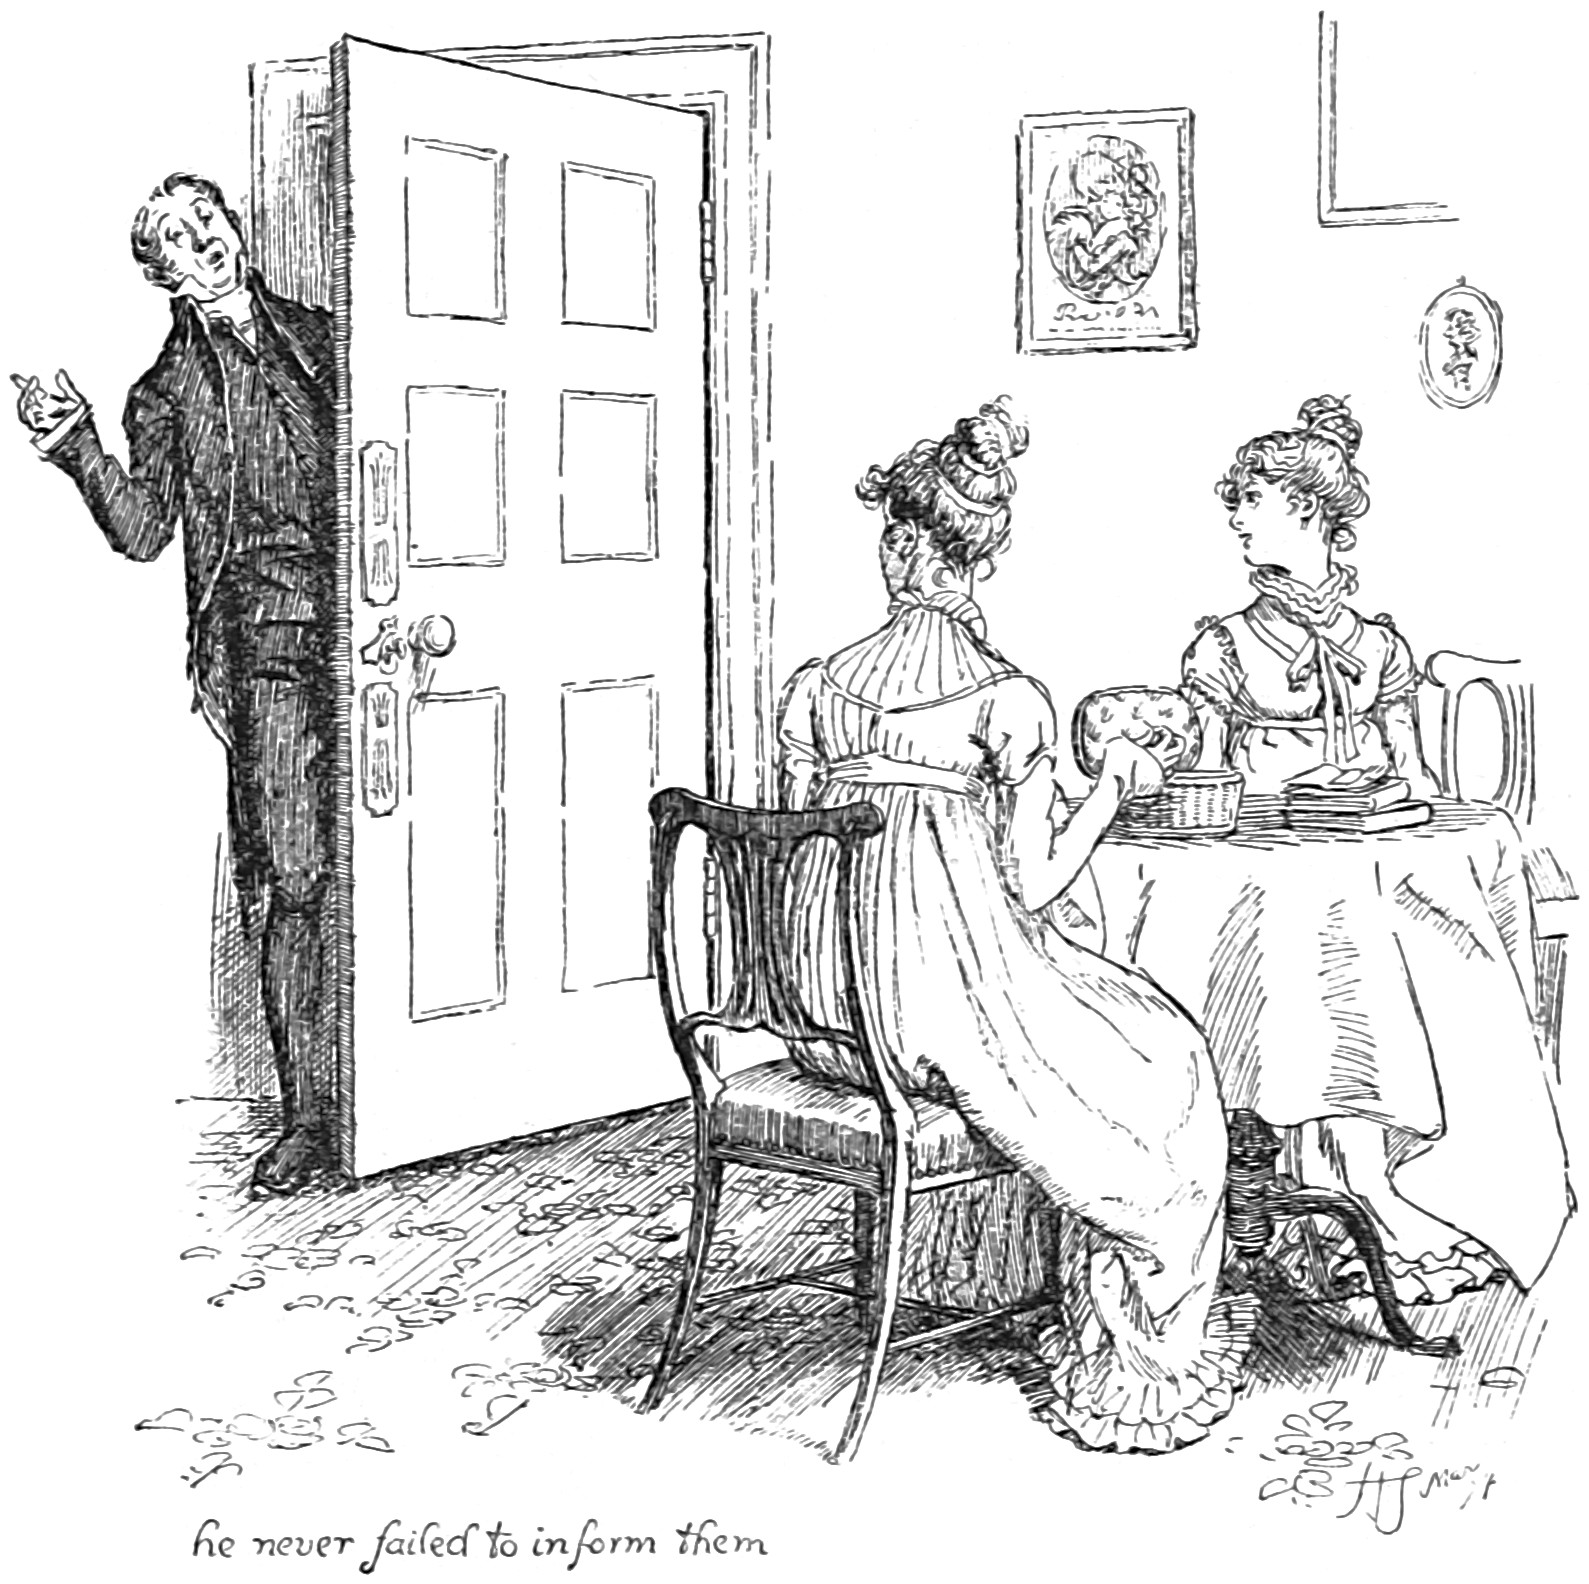
\includegraphics[width=\linewidth]{30inform}
\captionlistentry{He never failed to inform them}
\end{figure}

Very few days passed in which Mr Collins did not walk to Rosings, and not many in which his wife did not think it necessary to go likewise; and till Elizabeth recollected that there might be other family livings to be disposed of, she could not understand the sacrifice of so many hours. Now and then they were honoured with a call from her Ladyship, and nothing escaped her observation that was passing in the room during these visits. She examined into their employments, looked at their work, and advised them to do it differently; found fault with the arrangement of the furniture, or detected the housemaid in negligence; and if she accepted any refreshment, seemed to do it only for the sake of finding out that Mrs Collins's joints of meat were too large for her family.

Elizabeth soon perceived, that though this great lady was not in the commission of the peace for the county, she was a most active magistrate in her own parish, the minutest concerns of which were carried to her by Mr Collins; and whenever any of the cottagers were disposed to be quarrelsome, discontented, or too poor, she sallied forth into the village to settle their differences, silence their complaints, and scold them into harmony and plenty.

The entertainment of dining at Rosings was repeated about twice a week; and, allowing for the loss of Sir William, and there being only one card-table in the evening, every such entertainment was the counterpart of the first. Their other engagements were few, as the style of living of the neighbourhood in general was beyond the Collinses' reach. This, however, was no evil to Elizabeth, and upon the whole she spent her time comfortably enough: there were half hours of pleasant conversation with Charlotte, and the weather was so fine for the time of year, that she had often great enjoyment out of doors. Her favourite walk, and where she frequently went while the others were calling on Lady Catherine, was along the open grove which edged that side of the park, where there was a nice sheltered path, which no one seemed to value but herself, and where she felt beyond the reach of Lady Catherine's curiosity.

In this quiet way the first fortnight of her visit soon passed away. Easter was approaching, and the week preceding it was to bring an addition to the family at Rosings, which in so small a circle must be important. Elizabeth had heard, soon after her arrival, that Mr Darcy was expected there in the course of a few weeks; and though there were not many of her acquaintance whom she did not prefer, his coming would furnish one comparatively new to look at in their Rosings parties, and she might be amused in seeing how hopeless Miss Bingley's designs on him were, by his behaviour to his cousin, for whom he was evidently destined by Lady Catherine, who talked of his coming with the greatest satisfaction, spoke of him in terms of the highest admiration, and seemed almost angry to find that he had already been frequently seen by Miss Lucas and herself.

His arrival was soon known at the Parsonage; for Mr Collins was walking the whole morning within view of the lodges opening into Hunsford Lane, in order to have the earliest assurance of it; and, after making his bow as the carriage turned into the park, hurried home with the great intelligence. On the following morning he hastened to Rosings to pay his respects. There were two nephews of Lady Catherine to require them, for Mr Darcy had brought with him a Colonel Fitzwilliam, the younger son of his uncle, Lord ——; and, to the great surprise of all the party, when Mr Collins returned, the gentlemen accompanied him. Charlotte had seen them from her husband's room, crossing the road, and immediately running into the other, told the girls what an honour they might expect, adding,—

\begin{figure}[tbh]
\centering

\includegraphics[width=\linewidth]{30gentlemen}
\captionlistentry{The gentlemen accompanied him}
\end{figure}

»I may thank you, Eliza, for this piece of civility. Mr Darcy would never have come so soon to wait upon me.«

Elizabeth had scarcely time to disclaim all right to the compliment before their approach was announced by the door-bell, and shortly afterwards the three gentlemen entered the room. Colonel Fitzwilliam, who led the way, was about thirty, not handsome, but in person and address most truly the gentleman. Mr Darcy looked just as he had been used to look in Hertfordshire, paid his compliments, with his usual reserve, to Mrs Collins; and whatever might be his feelings towards her friend, met her with every appearance of composure. Elizabeth merely courtesied to him, without saying a word.

Colonel Fitzwilliam entered into conversation directly, with the readiness and ease of a well-bred man, and talked very pleasantly; but his cousin, after having addressed a slight observation on the house and garden to Mrs Collins, sat for some time without speaking to anybody. At length, however, his civility was so far awakened as to inquire of Elizabeth after the health of her family. She answered him in the usual way; and, after a moment's pause, added,—

»My eldest sister has been in town these three months. Have you never happened to see her there?«

She was perfectly sensible that he never had: but she wished to see whether he would betray any consciousness of what had passed between the Bingleys and Jane; and she thought he looked a little confused as he answered that he had never been so fortunate as to meet Miss Bennet. The subject was pursued no further, and the gentlemen soon afterwards went away.